\chapter{Conclusion}\label{chap:conclusion}

\section{Evaluation of Results}
To summarize the research conducted up to this point, a GPU-supported parallel Andersen based pointer analysis, PTAGPU was implemented on top of LLVM and the SVF framework using the NVIDIA CUDA SDK.
PTAGPU was both tested for correctness and performance in comparison to established CPU-based pointer analyses in multiple benchmarks and hardware combinations.
The primary research question was to what extent such an implementation presents advantages or disadvantages over other analyses that are not strictly parallel in nature.

\section{Future Work}
\subsection{Partitioning Workloads}
\subsection{Hybrid Cycle Detection}
\section{Discussion}

\appendix

\chapter{Raw Data}

\begin{table}[h]
    \tiny
    \begin{tabular}{rrrrrrrr}
        \toprule
           & file         & GPU memory MiB & filesize MB & wavediff-t   & naiveander-t & num nodes [K] & num edges [K] \\
        \midrule
        1  & bash         & 1024           & 5.400       & 16222.113    & 102195.752   & 238           & 77            \\
        2  & bison        & 260            & 3.400       & 18977.376    & 119999.054   & 146           & 59            \\
        3  & diff         & 71             & 1.300       & 1469.056     & 1561.577     & 54            & 17            \\
        4  & git          & 21467          & 25.000      & 557953.924   & 33404492.853 & 869           & 379           \\
        5  & htop         & 93             & 1.600       & 2912.693     & 5696.107     & 48            & 20            \\
        6  & httpd        & 160            & 1.400       & 5321.631     & 2889.208     & 169           & 95            \\
        7  & nano         & 7              & 0.298       & 87.438       & 98.500       & 6             & 2             \\
        8  & perl         & 3999           & 4.900       & 103338.824   & 2688610.846  & 445           & 206           \\
        9  & php          & 27561          & 52.000      & 645697.175   & 6530636.248  & 1582          & 611           \\
        10 & postgres     & 16430          & 18.000      & 997355.718   & 6481597.401  & 1432          & 721           \\
        11 & python       & 9016           & 21.000      & 536515.479   & 1731373.999  & 742           & 313           \\
        12 & redis-server & 207            & 4.800       & 8679.144     & 4834.759     & 207           & 67            \\
        13 & vim          & 11966          & 7.700       & 1052995.525  & NaN          & 696           & 280           \\
        14 & vmlinux      & NaN            & 72.000      & 32100566.652 & NaN          & 4464          & 2206          \\
        15 & vmlinux-tiny & 2175           & 5.400       & 91479.697    & 1410004.628  & 393           & 157           \\
        16 & zstd         & 454            & 2.300       & 11063.214    & 7958.999     & 280           & 101           \\
        \bottomrule
    \end{tabular}

    \caption{Raw Data of Baseline results for wavediff and naiveander Pointer Analyses}
\end{table}

\begin{table}[h]
    \tiny
    \begin{tabular}{rrrrrrrrrr}
        \toprule
           & ptagpu-t    & svf init & cuda init & update-k   & main-k       & thrust sort & store-k      & async CPU  & S    \\
        \midrule
        1  & 15489.00    & 366.515  & 2489.389  & 1129.063   & 1324.698     & 743.670     & 858.932      & 5190.693   & 1.05 \\
        2  & 9837.06     & 214.357  & 1650.840  & 830.177    & 234.046      & 675.748     & 54.633       & 4317.114   & 1.93 \\
        3  & 4231.58     & 66.945   & 2065.479  & 103.057    & 33.120       & 379.843     & 23.591       & 953.283    & 0.35 \\
        4  & 4690010.00  & 2190.250 & 17095.315 & 70148.000  & 3968158.215  & 11743.372   & 68373.295    & 538454.710 & 0.12 \\
        5  & 5275.51     & 68.425   & 2053.573  & 229.714    & 202.955      & 433.321     & 41.092       & 1587.968   & 0.55 \\
        6  & 6414.69     & 309.354  & 1481.509  & 303.996    & 42.605       & 511.057     & 8.219        & 1637.408   & 0.83 \\
        7  & 1751.01     & 7.732    & 1533.113  & 1.829      & 3.040        & 45.140      & 1.057        & 94.275     & 0.05 \\
        8  & 45093.40    & 775.915  & 2939.635  & 3457.350   & 6125.819     & 767.334     & 2751.206     & 21457.059  & 2.29 \\
        9  & 64965400.00 & 2809.670 & 20928.407 & 193679.543 & 53783100.092 & 12298.489   & 10732741.786 & 187398.213 & 0.01 \\
        10 & 465527.00   & 2911.590 & 8824.470  & 65379.251  & 192989.575   & 1374.555    & 32019.477    & 135372.093 & 2.14 \\
        11 & 203649.00   & 1344.910 & 4088.639  & 14380.164  & 63762.440    & 16295.704   & 12199.745    & 79598.063  & 2.63 \\
        12 & 11592.50    & 357.262  & 2785.032  & 688.684    & 95.318       & 1158.755    & 42.613       & 3688.319   & 0.75 \\
        13 & 268628.00   & 1166.830 & 9292.169  & 10709.775  & 113872.762   & 947.744     & 20876.445    & 100689.414 & 3.92 \\
        14 & NaN         & NaN      & NaN       & NaN        & NaN          & NaN         & NaN          & NaN        & NaN  \\
        15 & 188315.00   & 654.966  & 2405.784  & 10600.173  & 25890.805    & 12319.814   & 7893.207     & 121492.773 & 0.49 \\
        16 & 13172.60    & 388.764  & 2791.627  & 680.571    & 90.320       & 687.799     & 80.554       & 4526.521   & 0.84 \\
        \bottomrule
    \end{tabular}
    \caption{Raw Data of PTAGPU on Machine B}
\end{table}

\begin{table}[h]
    \tiny
    \begin{tabular}{rrrrrrrrrr}
        \toprule
           & ptagpu-t   & svf init & cuda init & update-k  & main-k     & thrust sort & store-k   & async CPU  & S    \\
        \midrule
        1  & 13126.316  & 316.589  & 3339.273  & 955.132   & 1258.228   & 103.923     & 824.671   & 3404.405   & 1.23 \\
        2  & 7599.453   & 181.425  & 3397.507  & 657.559   & 203.553    & 92.256      & 41.323    & 2941.927   & 2.49 \\
        3  & 3304.592   & 53.196   & 3119.867  & 100.198   & 29.448     & 73.122      & 13.813    & 379.511    & 0.44 \\
        4  & 869302.000 & 1489.250 & 2852.620  & 31480.079 & 350891.929 & 4856.937    & 30923.576 & 431554.218 & 0.64 \\
        5  & 4038.684   & 58.770   & 3238.629  & 212.349   & 189.568    & 74.528      & 20.536    & 852.136    & 0.72 \\
        6  & 4720.701   & 233.173  & 3125.778  & 258.309   & 39.757     & 57.139      & 5.049     & 848.704    & 1.12 \\
        7  & 1626.456   & 5.655    & 3163.307  & 2.024     & 4.073      & 8.778       & 0.786     & 18.179     & 0.05 \\
        8  & 41853.936  & 644.417  & 3277.899  & 3452.222  & 6873.348   & 164.523     & 2906.182  & 18027.103  & 2.46 \\
        9  & 500086.000 & 2561.200 & 3815.678  & 32016.810 & 184075.139 & 2797.468    & 49062.434 & 198397.500 & 1.29 \\
        10 & 290219.000 & 2465.070 & 4439.149  & 12040.787 & 140270.103 & 211.504     & 14064.883 & 89735.395  & 3.43 \\
        11 & 172701.000 & 1088.500 & 3468.036  & 14790.821 & 65522.991  & 203.848     & 11336.972 & 63986.167  & 3.10 \\
        12 & 8830.066   & 247.339  & 3339.556  & 615.407   & 103.871    & 109.152     & 24.580    & 2143.869   & 0.98 \\
        13 & 247859.000 & 963.959  & 3336.741  & 7599.231  & 125708.265 & 123.820     & 23102.001 & 75995.761  & 4.24 \\
        14 & NaN        & NaN      & NaN       & NaN       & NaN        & NaN         & NaN       & NaN        & NaN  \\
        15 & 136164.602 & 554.447  & 3152.182  & 11286.157 & 26563.670  & 236.409     & 8721.936  & 79417.327  & 0.67 \\
        16 & 9795.036   & 312.077  & 3104.891  & 546.614   & 70.509     & 75.957      & 61.621    & 2587.828   & 1.12 \\
        \bottomrule
    \end{tabular}
    \caption{Raw Data of PTAGPU on Machine C}
\end{table}
\normalsize

\begin{figure}[h]
    \centering
    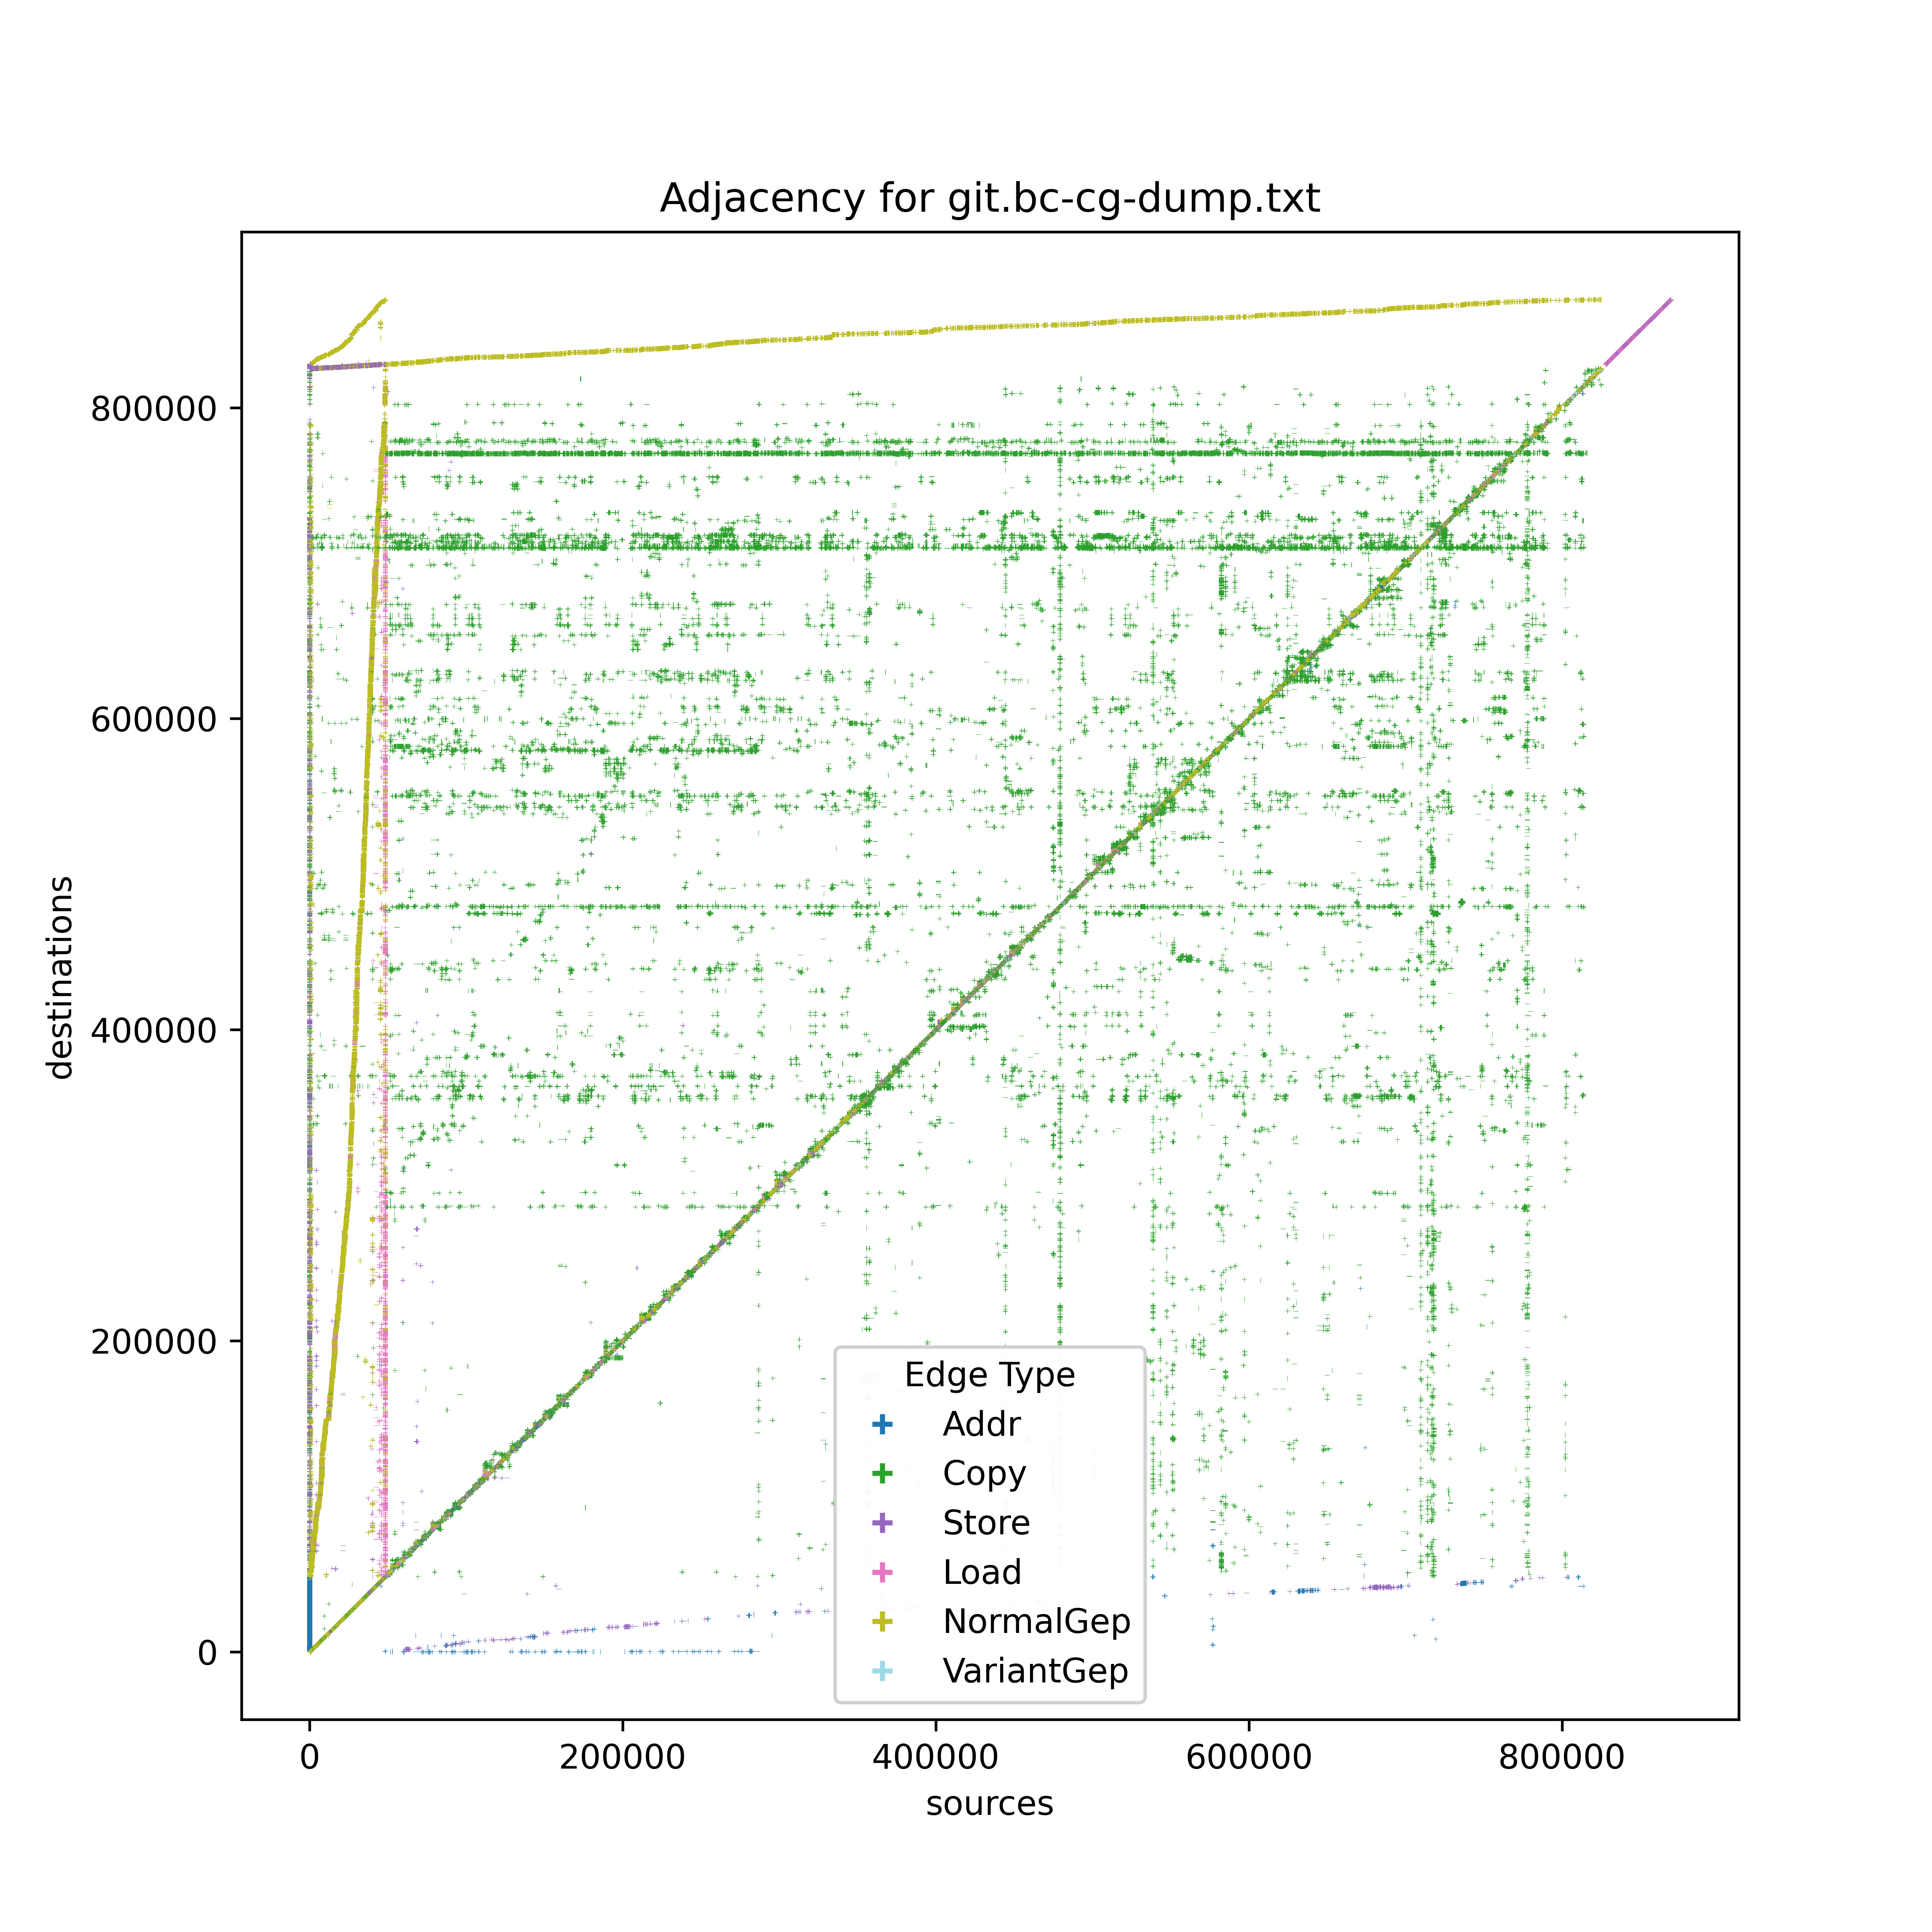
\includegraphics[width=.7\textwidth]{img/plot-git.bc-cg-dump.txt-min.png}
    \caption{Adjacency Plot for the Constraint Graph of the Git Client}
    \label{fig:git-consg}
\end{figure}

\begin{figure}[h]
    \centering
    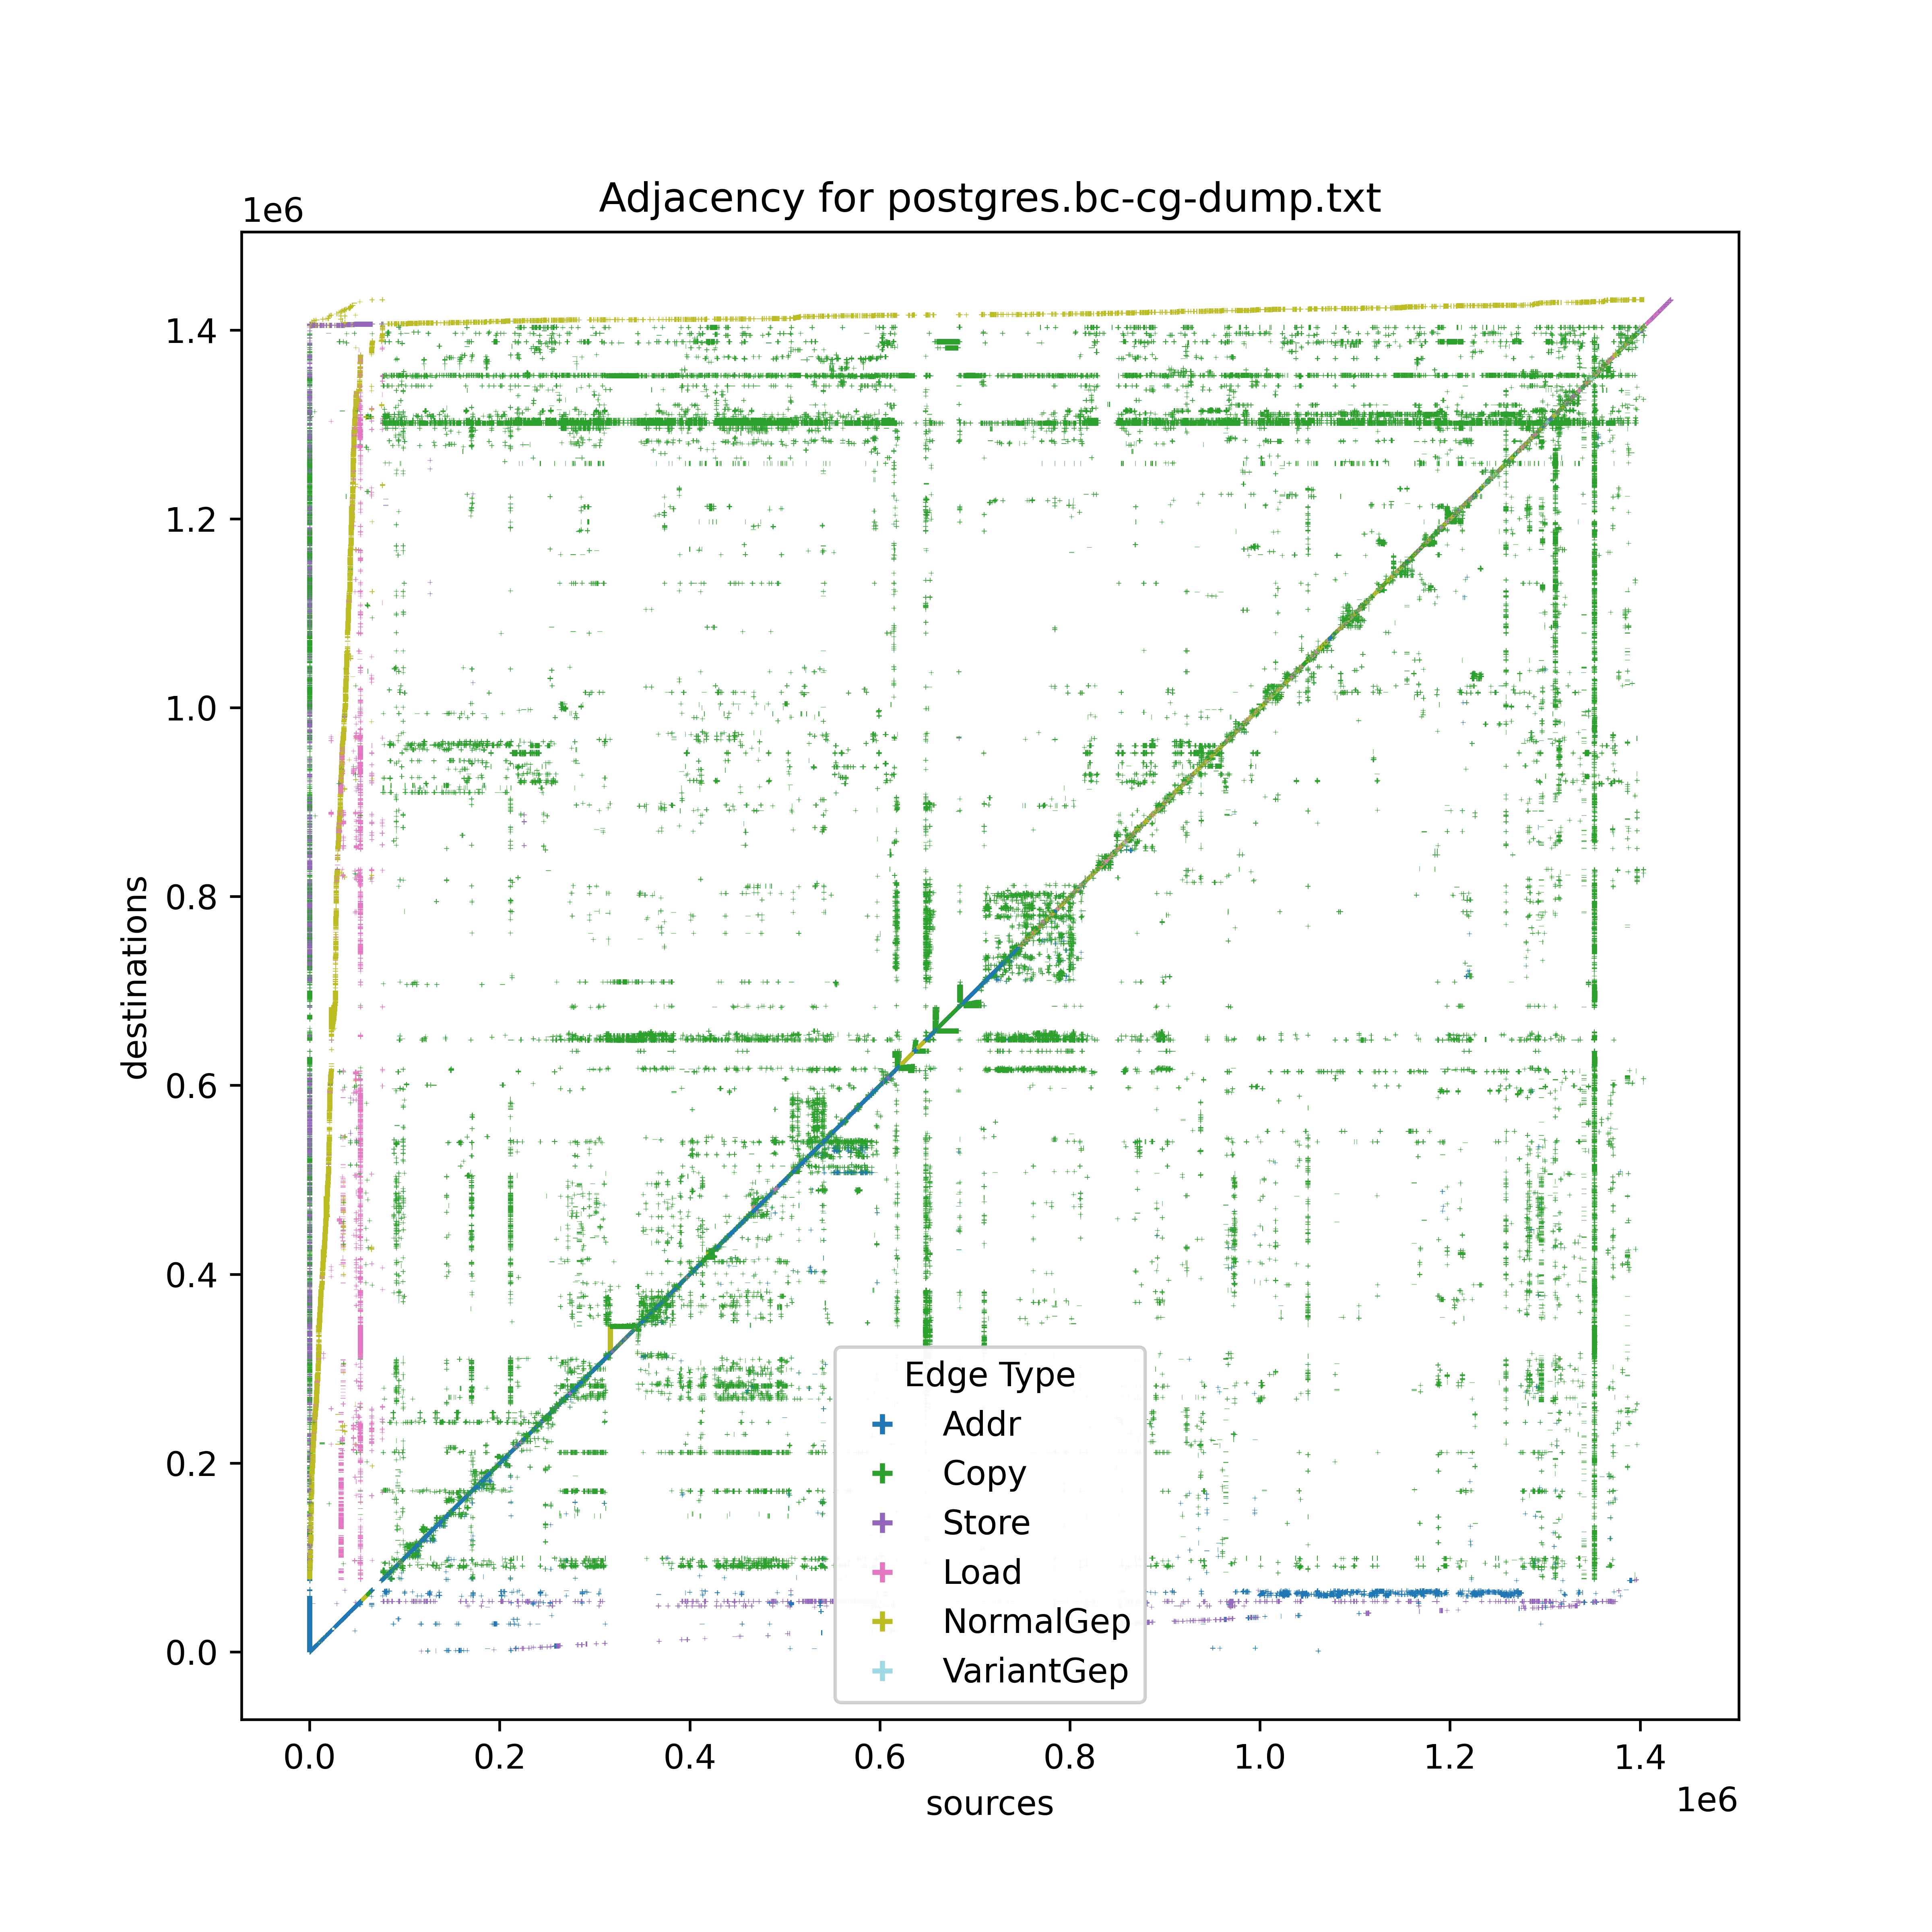
\includegraphics[width=.7\textwidth]{img/plot-postgres.bc-cg-dump.txt-min.png}
    \caption{Adjacency Plot for the Constraint Graph of Postgres}
    \label{fig:postgres-consg}
\end{figure}